\documentclass{beamer}

\usepackage{beamerthemeCambridgeUS}
\usepackage{textpos}
\usepackage{ragged2e}
\usepackage{ulem}

\graphicspath{{G:/My Drive/FIGURAS/}}

\title[Sistemas de Clasificación Geomorfológica]{GEOMORFOLOGÍA}
\author[Edier Aristizabal]{Edier V. Aristizábal G.}
\institute{evaristizabalg@unal.edu.co}
\date{\tiny{Versión:\today}}

\addtobeamertemplate{headline}{}{%
	\begin{textblock*}{2mm}(.9\textwidth,0cm)
	\hfill\includegraphics[height=1cm]{un}  
	\end{textblock*}}

\begin{document}
%%%%%%%%%%%%%%%%%%%%%%%%%%%%%%%%%%%%%%%%%%%%%%%%%%%%%%%%%%%%%%%%%%%%%%%%%
\begin{frame}
\titlepage
\centering
   	\includegraphics[width=4cm]{unal} 
\end{frame}
%%%%%%%%%%%%%%%%%%%%%%%%%%%%%%%%%%%%%%%%%%%%%%%%%%%%%%%%%%%%%%%%%%%%%%%%%
\begin{frame}
\frametitle{Metodologia}
\begin{center}
   	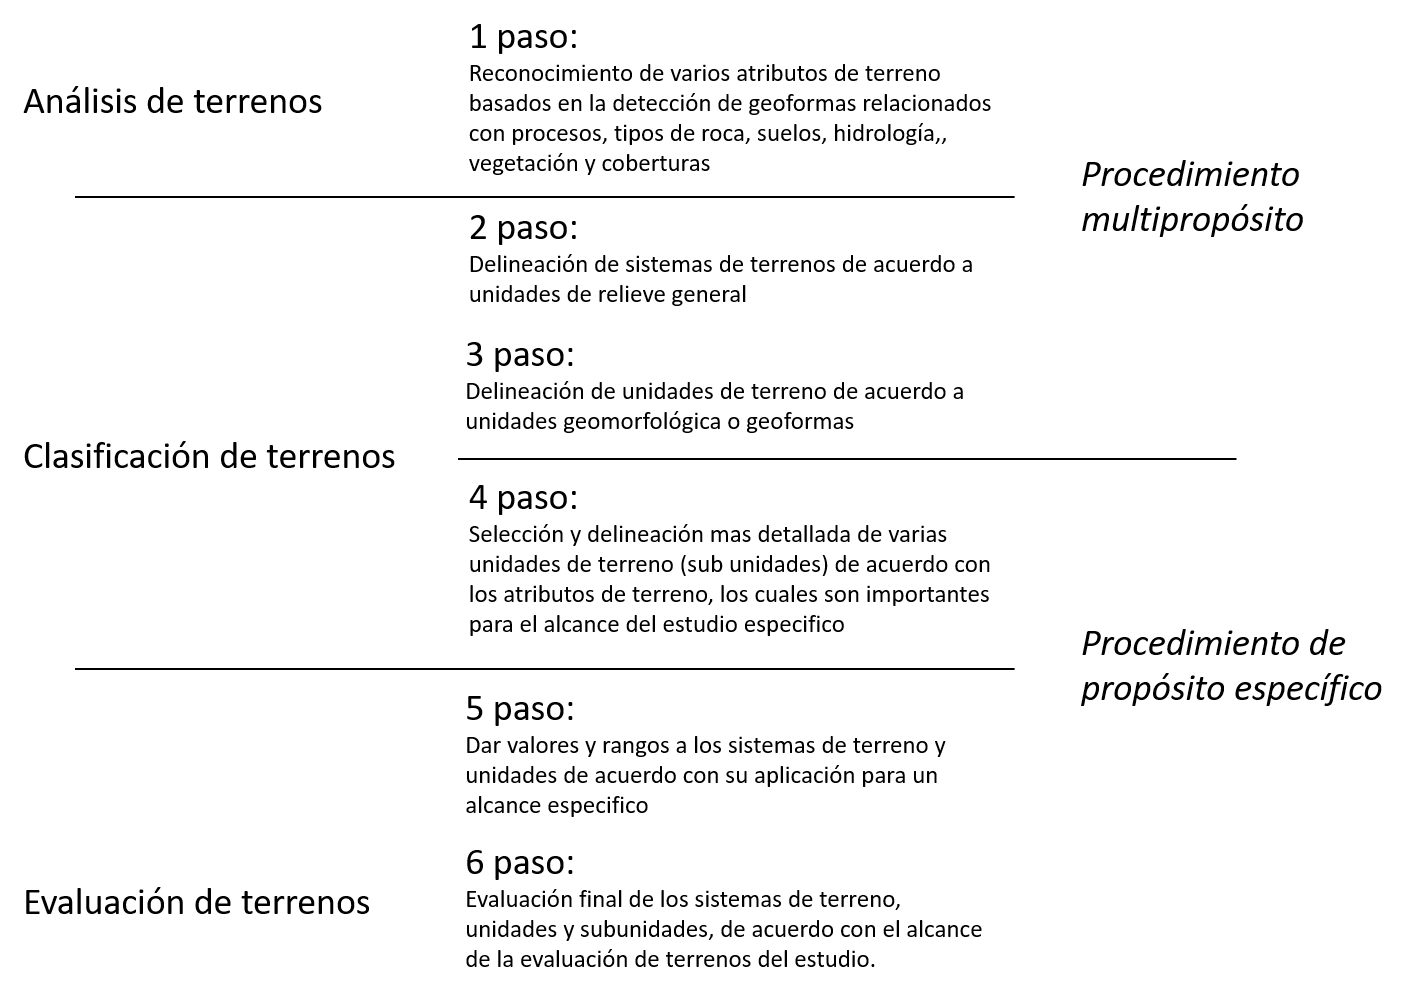
\includegraphics[scale=0.45]{metocarto}
\end{center}
\end{frame}
%%%%%%%%%%%%%%%%%%%%%%%%%%%%%%%%%%%%%%%%%%%%%%%%%%%%%%%%%%%%%%%%%%%%%%%%%
\begin{frame}
\frametitle{Mapa geomorfológico analítico}
\begin{center}
   	\includegraphics[scale=0.45]{mapageomorfologico1}
\end{center}
\end{frame}
%%%%%%%%%%%%%%%%%%%%%%%%%%%%%%%%%%%%%%%%%%%%%%%%%%%%%%%%%%%%%%%%%%%%%%%%%
\begin{frame}
\frametitle{Mapa geomorfológico pragmático}
\begin{center}
   	\includegraphics[scale=0.45]{mapageomorfologico4}
\end{center}
\tiny{Fuente: van Westen et al. (2003)}
\end{frame}
%%%%%%%%%%%%%%%%%%%%%%%%%%%%%%%%%%%%%%%%%%%%%%%%%%%%%%%%%%%%%%%%%%%%%%%%%
\begin{frame}
\frametitle{Clasificación taxonómica de unidades}
\begin{center}
   	\includegraphics[scale=0.45]{tricart}
\end{center}
\tiny{Fuente: Modificado de Tricart (1965)  en Zinck (2012)}
\end{frame}
%%%%%%%%%%%%%%%%%%%%%%%%%%%%%%%%%%%%%%%%%%%%%%%%%%%%%%%%%%%%%%%%%%%%%%%%%
\begin{frame}
\frametitle{Clasificación taxonómica de unidades}
\begin{center}
   	\includegraphics[scale=0.45]{zink}
\end{center}
\tiny{Fuente: Zinck (1988)}
\end{frame}
%%%%%%%%%%%%%%%%%%%%%%%%%%%%%%%%%%%%%%%%%%%%%%%%%%%%%%%%%%%%%%%%%%%%%%%%%
\begin{frame}
\frametitle{Geoformas de relieve y modelado}
\small{
\textbf{Relieve}: Geoforma que resulta de una determinada combinación de topografía y estructura controlada mayormente por la geodinámica interna. Ej. Cuesta.\\
\textbf{Modelado}: Geoforma determinada por condiciones morfoclimáticas o proceso morfogenéticos controlada mayormente por la geodinámica externa. Ej. Terraza.
}
\begin{center}
   	\includegraphics[scale=0.451]{relievemodelado}
\end{center}
\tiny{Fuente: Zinck (1988)}
\end{frame}
%%%%%%%%%%%%%%%%%%%%%%%%%%%%%%%%%%%%%%%%%%%%%%%%%%%%%%%%%%%%%%%%%%%%%%%%%
\begin{frame}
\frametitle{Modelado Glacial}
\begin{center}
	\includegraphics[scale=0.5]{modeladoglacial}
   	\includegraphics[scale=0.3]{glaciar2}
\end{center}
\tiny{Fuente: Zinck (1988)}
\end{frame}
%%%%%%%%%%%%%%%%%%%%%%%%%%%%%%%%%%%%%%%%%%%%%%%%%%%%%%%%%%%%%%%%%%%%%%%%%
\begin{frame}
\frametitle{Niveles de percepción de geoformas}
\begin{center}
	\includegraphics[scale=0.5]{nivelespercepcion}
\end{center}
\tiny{Fuente: Zinck (1988)}
\end{frame}
%%%%%%%%%%%%%%%%%%%%%%%%%%%%%%%%%%%%%%%%%%%%%%%%%%%%%%%%%%%%%%%%%%%%%%%%%
\begin{frame}
\frametitle{Niveles de percepción de geoformas}
\begin{center}
	\includegraphics[scale=0.4]{nivelespercepcion1}
\end{center}
\tiny{Fuente: Zinck (1988)}
\end{frame}
%%%%%%%%%%%%%%%%%%%%%%%%%%%%%%%%%%%%%%%%%%%%%%%%%%%%%%%%%%%%%%%%%%%%%%%%%
\begin{frame}
\frametitle{Sistemas de terreno jerárquico}
\begin{columns}
\begin{column}{0.4\textwidth}
\begin{center}
	\includegraphics[scale=0.7]{wielemaker}
\end{center}
\tiny{Fuente: Wielemaker et al (2001)}
\end{column}
\begin{column}{0.6\textwidth}
	\scriptsize{\textbf{Región}: Área con un patrón de geoformas mayores compartiendo una historia geológica común. Escala $1:1.000.000 a 1: 5.000.000$. Región volcánica, región costera, región montañosa.\\
\textbf{Geoforma Mayor}: un patrón de uno o mas unidades de clases de elementos de geoformas compartiendo una morfogénesis principal. Tiene un tipo de relieve particular y posición y un patrón de formas que refleja la naturaleza y composición de sus partes. Escala $1:50.000 a 1: 200.000$. Plano aluvial de piedemonte, montañas metamórficas.\\
\textbf{Elemento de Geoforma}: la más detallada unidad geomorfológica de la cual la Geoforma Mayor está compuesta. Se clasifica basado en un proceso genético particular y litológico. El patrón de ladera puede ser adicionado como un criterio. Escala $1: 20.000 a 1: 50.000$. Terraza de riso recientes.\\
\textbf{Faceta}: componente del Elemento de Geoforma, uniforme en términos de topografía; su mínimo tamaño es acerca de 200 m2. escala $1:5.000 a 1:20.000$.\\
\textbf{Sitio nivel pedon}. Área con radio de 7 m, donde el terreno las características del perfil son levantadas. El perfil es subdividido en capas u horizontes.
}
\end{column}
\end{columns}
\end{frame}
%%%%%%%%%%%%%%%%%%%%%%%%%%%%%%%%%%%%%%%%%%%%%%%%%%%%%%%%%%%%%%%%%%%%%%%%%
\begin{frame}
\frametitle{Niveles de percepción de geoformas}
\begin{center}
	\includegraphics[scale=0.65]{wielemaker1}
\end{center}
\tiny{Fuente: Wielemaker et al (2001)}
\end{frame}
%%%%%%%%%%%%%%%%%%%%%%%%%%%%%%%%%%%%%%%%%%%%%%%%%%%%%%%%%%%%%%%%%%%%%%%%%
\begin{frame}
\frametitle{Niveles de percepción de geoformas}
\begin{center}
	\includegraphics[scale=0.55]{wielemaker2}
\end{center}
\tiny{Fuente: Wielemaker et al (2001)}
\end{frame}
%%%%%%%%%%%%%%%%%%%%%%%%%%%%%%%%%%%%%%%%%%%%%%%%%%%%%%%%%%%%%%%%%%%%%%%%%
\begin{frame}
\frametitle{Niveles de percepción de geoformas}
\begin{center}
	\includegraphics[scale=0.45]{wielemaker3}
\end{center}
\tiny{Fuente: Wielemaker et al (2001)}
\end{frame}
%%%%%%%%%%%%%%%%%%%%%%%%%%%%%%%%%%%%%%%%%%%%%%%%%%%%%%%%%%%%%%%%%%%%%%%%%
\begin{frame}
\frametitle{\emph{Terrain \& Land}}
\small{
\textbf{Fisiografía} = estudio de la génesis y evolución de las formas de \emph{land forms} $\rightarrow$ vegetación y uso del suelo. La fisiografía no solo describe los aspectos relativos a la litosfera (relieve, materiales, edad de las formaciones superficiales, proceso morfogenéticos), como lo hace la geomorfología, sino que también describe los relativos al agua, el clima y los seres vivos.\\
\vspace{5pt}
\textbf{Terrain}
\begin{itemize}
\item Describe una división natural del terreno que puede ser distinguida en fotografías aéreas y que puede ser verificada en campo.\\
\item Es una unidad donde los grupos se interrelacionan en términos de geoformas, litología y suelo.\\
\item Difiere de la otras unidades por que las geoformas son evidentemente diferentes o los fenómenos asociados con la geoformas difieren.\
\item En términos de GIS puede ser descrita como la localización geográfica en polígonos o entidades en las cuales se relacionan un único grupo de atributos.\\
\item Es una unidad de leyenda de un mapa temático convencional.
\end{itemize}
}
\tiny{Fuente: Meijerink (1988)}
\end{frame}
%%%%%%%%%%%%%%%%%%%%%%%%%%%%%%%%%%%%%%%%%%%%%%%%%%%%%%%%%%%%%%%%%%%%%%%%%
\begin{frame}
\frametitle{Clasificación fisiográfica}
\begin{columns}
\begin{column}{0.5\textwidth}
\begin{center}
	\includegraphics[scale=0.5]{serrato}
\end{center}
\tiny{Fuente: Serrato(2009)}
\end{column}
\begin{column}{0.5\textwidth}
	\begin{center}
	\includegraphics[scale=0.55]{serrato1}
\end{center}
\end{column}
\end{columns}
\end{frame}
%%%%%%%%%%%%%%%%%%%%%%%%%%%%%%%%%%%%%%%%%%%%%%%%%%%%%%%%%%%%%%%%%%%%%%%%%
\begin{frame}
\frametitle{Provincia fisiográfica}
\begin{center}
	\includegraphics[scale=0.4]{provincia}
\end{center}
\tiny{Fuente: Serrato(2009)}
\end{frame}
%%%%%%%%%%%%%%%%%%%%%%%%%%%%%%%%%%%%%%%%%%%%%%%%%%%%%%%%%%%%%%%%%%%%%%%%%
\begin{frame}
\frametitle{Unidad climática}
\begin{center}
	\includegraphics[scale=0.5]{unidadclimatica}
\end{center}
\end{frame}
%%%%%%%%%%%%%%%%%%%%%%%%%%%%%%%%%%%%%%%%%%%%%%%%%%%%%%%%%%%%%%%%%%%%%%%%%
\begin{frame}
\frametitle{Gran Paisaje}
\begin{center}
	\includegraphics[scale=0.5]{granpaisaje}
\end{center}
\end{frame}
%%%%%%%%%%%%%%%%%%%%%%%%%%%%%%%%%%%%%%%%%%%%%%%%%%%%%%%%%%%%%%%%%%%%%%%%%
\begin{frame}
\frametitle{Paisaje Fisiográfico}
\begin{center}
	\includegraphics[scale=0.5]{paisajefisio}
\end{center}
\end{frame}
%%%%%%%%%%%%%%%%%%%%%%%%%%%%%%%%%%%%%%%%%%%%%%%%%%%%%%%%%%%%%%%%%%%%%%%%%
\begin{frame}
\frametitle{Subpaisaje Fisiográfico}
\begin{center}
	\includegraphics[scale=0.55]{subpaisajefisio}
\end{center}
\end{frame}
%%%%%%%%%%%%%%%%%%%%%%%%%%%%%%%%%%%%%%%%%%%%%%%%%%%%%%%%%%%%%%%%%%%%%%%%%
\begin{frame}
\frametitle{Metodología IDEAM 1:100.000}
\begin{center}
	\includegraphics[scale=0.55]{metodologiaIDEAM}
\end{center}
\end{frame}
%%%%%%%%%%%%%%%%%%%%%%%%%%%%%%%%%%%%%%%%%%%%%%%%%%%%%%%%%%%%%%%%%%%%%%%%%
\begin{frame}
\frametitle{Metodología ITC}
\justifying
\small{La clasificación de terrenos corresponde al arreglo y agrupamiento de diferentes áreas de la superficie terrestre en una variedad de categorías (provincia, sistema, unidades y componentes) basados en la similitud de los atributos,  tipo de superficie y sus alrededores.
}
\begin{center}
	\includegraphics[scale=0.45]{itc}
\end{center}
\tiny{Fuente: van Zuidam (1985)}
\end{frame}
%%%%%%%%%%%%%%%%%%%%%%%%%%%%%%%%%%%%%%%%%%%%%%%%%%%%%%%%%%%%%%%%%%%%%%%%%
\begin{frame}
\frametitle{Metodología SGC}
\begin{center}
	\includegraphics[scale=0.50]{sgc_metodologia}
\end{center}
\tiny{Fuente: Velásquez (1999); Ingeominas (2000)}
\end{frame}
%%%%%%%%%%%%%%%%%%%%%%%%%%%%%%%%%%%%%%%%%%%%%%%%%%%%%%%%%%%%%%%%%%%%%%%%%
\begin{frame}
\frametitle{Metodología SGC}
\begin{center}
	\includegraphics[scale=0.45]{sgc_metodologia1}
\end{center}
\tiny{Fuente: Ingeominas (2000)}
\end{frame}
%%%%%%%%%%%%%%%%%%%%%%%%%%%%%%%%%%%%%%%%%%%%%%%%%%%%%%%%%%%%%%%%%%%%%%%%%
\begin{frame}
\frametitle{Morfogenética}
\begin{center}
	\includegraphics[scale=0.45]{itcsgc}
\end{center}
\end{frame}
%%%%%%%%%%%%%%%%%%%%%%%%%%%%%%%%%%%%%%%%%%%%%%%%%%%%%%%%%%%%%%%%%%%%%%%%%
\begin{frame}
\frametitle{Catálogo del SGC (1:100.000)}
\begin{center}
	\includegraphics[scale=0.45]{catalogo100k}
\end{center}
\end{frame}
%%%%%%%%%%%%%%%%%%%%%%%%%%%%%%%%%%%%%%%%%%%%%%%%%%%%%%%%%%%%%%%%%%%%%%%%%
\begin{frame}
\frametitle{Geoformas banales}
\small{Que no presentan geoformas rasgos fisiográficos particularmente resaltantes. }
\begin{center}
	\includegraphics[scale=0.55]{banales}
\end{center}
\tiny{Fuente: Zinck (1988)}
\end{frame}
%%%%%%%%%%%%%%%%%%%%%%%%%%%%%%%%%%%%%%%%%%%%%%%%%%%%%%%%%%%%%%%%%%%%%%%%%
\end{document}